\documentclass[11pt]{article}
\usepackage{amsmath,amssymb,amsthm}
\usepackage[margin=1.1in]{geometry}
\usepackage{booktabs}
\usepackage{graphicx}
\emergencystretch=1.5em

\newtheorem{theorem}{Theorem}[section]
\newtheorem{conjecture}[theorem]{Conjecture}
\theoremstyle{remark}
\newtheorem{remark}[theorem]{Remark}
\newtheorem{observation}[theorem]{Observation}

\newcommand{\R}{\mathbb{R}}

\title{Zeros of the Polynomial Sections of Hermite Functions:\\
a Szeg\H{o}-Type Limit Curve}
\author{Robin Langer and Claude Code}
\date{August 2026}

\begin{document}
\maketitle

\begin{abstract}
The $L^2(\R, e^{-t^2}dt)$-projection of the Hermite function $\psi_m$ onto polynomials of degree $\le N$ is a polynomial $\psi_m^{(N)}$ with (up to one universal constant) rational coefficients. We compute its zeros exactly for $m = 0, 4$ and $N \le 320$. The $m$ genuine zeros of $\psi_m$ are captured rapidly; the $N - m$ spurious zeros split into two families: real zeros densely filling a band $\alpha \le |t|/\sqrt{2N} \le 1$, and two complex arcs. This differs from the classical Szeg\H{o} picture for the Taylor sections of $e^z$, where no spurious zeros are real. We conjecture that the onset of the real band is
\[
\alpha = \tfrac{1}{2}\sqrt{\ln 3} = 0.5241\ldots,
\]
equivalently: real spurious zeros begin where the \emph{weight} $e^{-t^2}$ equals the coefficient decay $3^{-N/2}$. Numerics for $N \le 320$ agree, including the predicted $O(\ln N / N)$ finite-size correction.
\end{abstract}

\section{Setup}

Let $\psi_m(t) = c_m H_m(t) e^{-t^2/2}$ be the Hermite functions and let
\[
\psi_m^{(N)}(t) = \sum_{k=0}^{N} a_{mk} H_k(t)
\]
be the best $L^2(\R, e^{-t^2}dt)$-approximation of $\psi_m$ by a polynomial of degree $\le N$, as in our companion paper on the Hermite matching matrix. Up to the universal constant $\sqrt{2/3}/\pi^{1/4}$ the coefficients are rational; for $m = 0$,
\begin{equation}
\psi_0^{(N)}(t) \;\propto\; \sum_{n=0}^{\lfloor N/2 \rfloor} \frac{(-1)^n}{n!\, 12^n}\, H_{2n}(t).
\label{eq:m0}
\end{equation}
In the orthonormal normalisation the coefficients decay geometrically: $b_k := a_{mk}\|H_k\| \sim \rho^k$ with $\rho = 1/\sqrt{3}$, times a polynomial factor (of degree growing with $m$). Consequently $\psi_m^{(N)} \to \psi_m$ locally uniformly, and by Hurwitz the $m$ real zeros of $H_m$ persist. The remaining $N - m$ zeros must escape to infinity; the question is how.

All computations below use exact rational arithmetic for the coefficients (the corrected matching matrix, cross-pair weight $+4$) and multiprecision root-finding, verified by exact evaluation at the computed roots.

\section{The three families of zeros}

Figure~\ref{fig:zeros} shows the zeros of $\psi_0^{(N)}$ for $N = 20, \dots, 56$, scaled by $1/\sqrt{2N}$, and of $\psi_4^{(40)}$ unscaled.

\begin{figure}[ht]
\centering
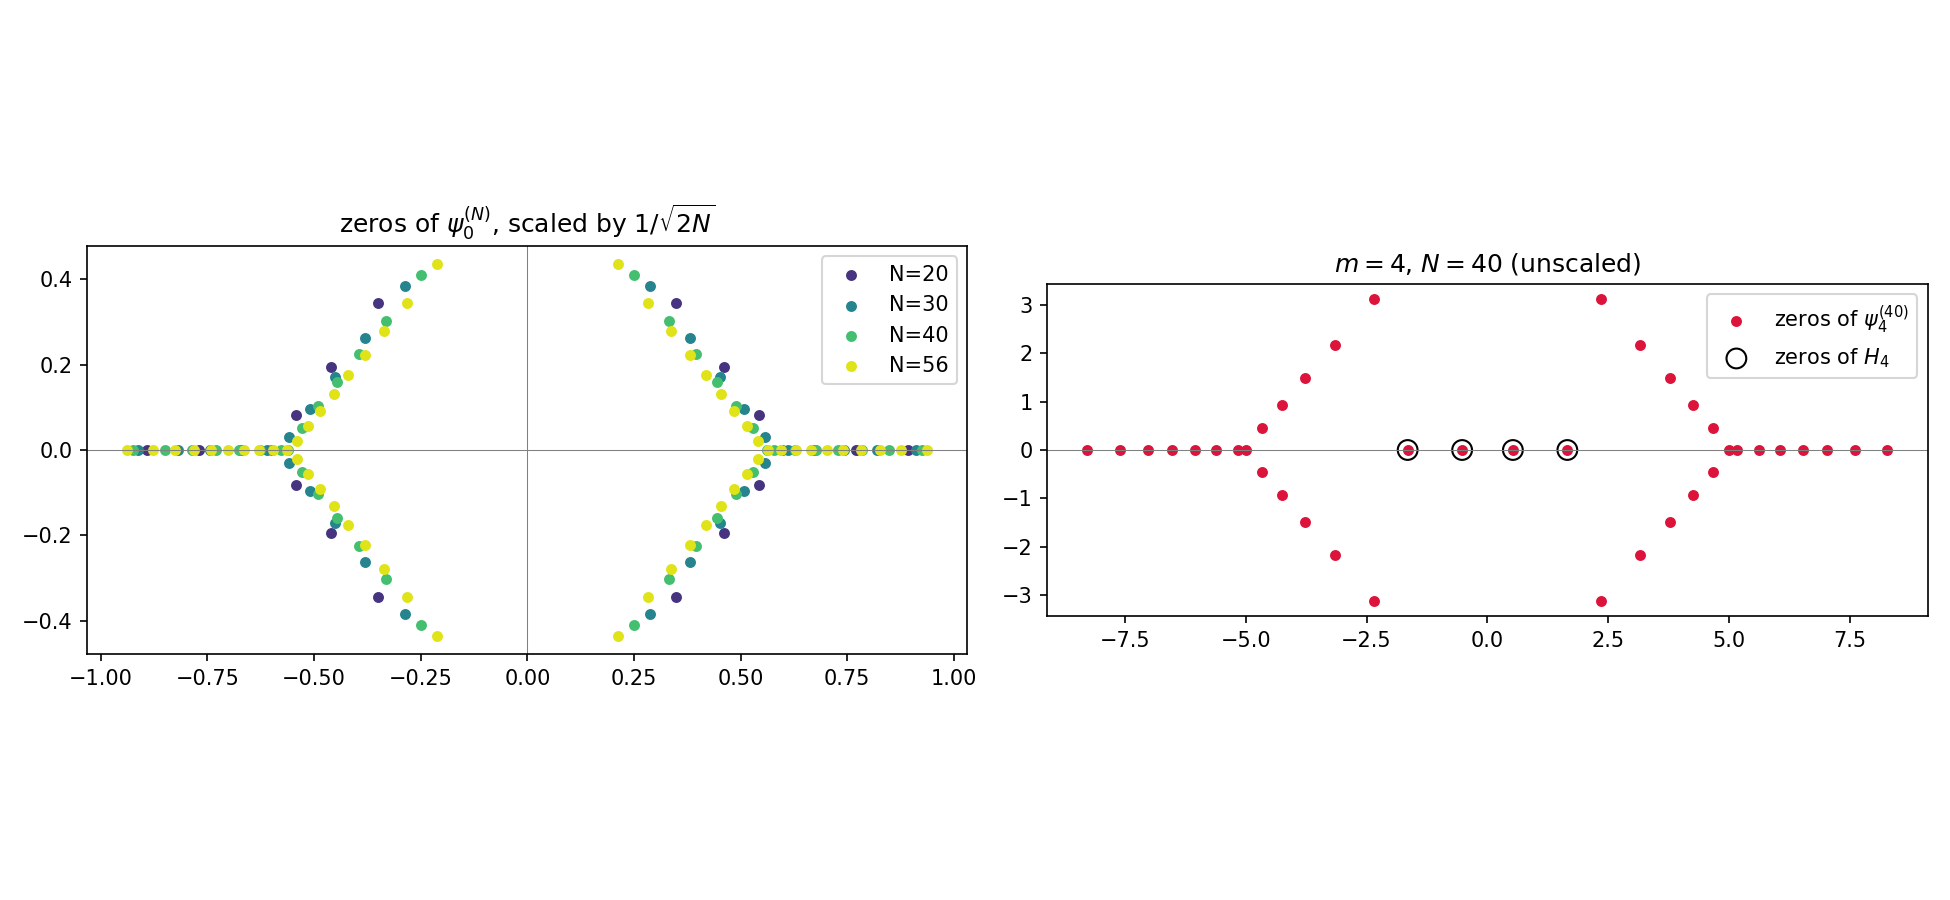
\includegraphics[width=\textwidth]{approximant_zeros.png}
\caption{Left: zeros of $\psi_0^{(N)}$ in the scaled variable $w = t/\sqrt{2N}$; the sets for different $N$ collapse onto a single limiting shape. Right: zeros of $\psi_4^{(40)}$; circles mark the zeros of $H_4$.}
\label{fig:zeros}
\end{figure}

\begin{observation}
Three families are visible.
\begin{enumerate}
\item \textbf{Genuine zeros.} For $m = 4$, $N = 40$, four zeros of $\psi_4^{(N)}$ agree with the zeros of $H_4$ ($\pm 0.5246487$, $\pm 1.6506801$) to six decimal places.
\item \textbf{Real spurious zeros.} The remaining real zeros fill a band $\alpha_N \le |w| \le \beta_N$ with $\alpha_N \approx 0.53$--$0.56$ (slowly decreasing in $N$) and $\beta_N \to 1$ from below, consistent with an Airy-type edge $1 - \beta_N = O(N^{-2/3})$ (measured $0.90, 0.92, 0.94, 0.95$ for $N = 24, 40, 56, 72$).
\item \textbf{Complex arcs.} Two arcs leave the real axis near $\pm\alpha_N$ and terminate near $\pm(0.21 \pm 0.44 i)$, stable in the scaled variable.
\end{enumerate}
\end{observation}

No spurious zeros are real for the Taylor sections of $e^z$ (Szeg\H{o}); here a positive fraction of them are. The mechanism is identified in the next section.

\section{The crossover mechanism}

Write $\psi_0^{(N)} = L - T_N$ with limit $L(t) = \sqrt{3/2}\, e^{-t^2/2}$ (in the normalisation of \eqref{eq:m0}) and tail $T_N(t) = \sum_{k > N} a_{0k} H_k(t)$. The key elementary point is that the tail is a series in Hermite \emph{polynomials}, not Hermite functions:
\[
a_k H_k(t) = b_k\, \psi_k(t)\, e^{t^2/2}, \qquad b_k \sim \rho^k = 3^{-k/2},
\]
and $|\psi_k| = O(1)$ uniformly. Hence for real $t$ in the oscillatory range of the tail modes,
\begin{equation}
|T_N(t)| \;\asymp\; 3^{-N/2}\, e^{t^2/2} \quad\text{(up to powers of $N$)}.
\label{eq:tail}
\end{equation}
The tail \emph{grows} like the inverse square root of the weight. Spurious real zeros appear exactly where the oscillating tail dominates the target: $|T_N| \gtrsim |L|$, i.e.
\[
3^{-N/2} e^{t^2/2} \;\ge\; e^{-t^2/2}
\quad\Longleftrightarrow\quad
e^{-t^2} \le 3^{-N/2}
\quad\Longleftrightarrow\quad
|t| \ge \sqrt{\tfrac{N}{2}\ln 3}.
\]
In the scaled variable this reads $|w| \ge \frac12\sqrt{\ln 3} = 0.52413\ldots$ The onset is where the \emph{weight of the inner product} equals the $N$-th power of the coefficient ratio: $e^{-t^2} = \rho^{2N}$. Beyond the onset $\psi_0^{(N)} \approx -T_N$ oscillates like its top Hermite mode, producing real zeros with locally Hermite spacing, out to the turning point $w = 1$.

Refining \eqref{eq:tail} with the bulk amplitude $|\psi_N| \sim N^{-1/4}$ gives the finite-size prediction
\begin{equation}
\alpha_N^2 \;=\; \tfrac{\ln 3}{4} + \tfrac{\ln N}{8N} + O(1/N).
\label{eq:correction}
\end{equation}

Locating $\alpha_N$ directly as the crossing $|{\psi_0^{(N)} - L}| = |L|$ (exact rational evaluation, no root-finding):

\begin{center}
\begin{tabular}{lcccc}
\toprule
$N$ & $40$ & $80$ & $160$ & $320$ \\
\midrule
$\alpha_N$ (measured) & $0.5615$ & $0.5452$ & $0.5384$ & $0.5321$ \\
$\alpha_N$ from \eqref{eq:correction} & $0.535$ & $0.531$ & $0.528$ & $0.526$ \\
\bottomrule
\end{tabular}
\end{center}

The measured values decrease monotonically toward $\frac12\sqrt{\ln 3} = 0.5241$, with a residual gap shrinking like the neglected $O(1/N)$ terms.

\section{The conjecture}

Let $Z_N \subset \mathbb{C}$ be the zero set of $\psi_m^{(N)}$, scaled by $1/\sqrt{2N}$, and let $\mu_N$ be its counting measure normalised by $N$.

\begin{conjecture}[Szeg\H{o} curve for Hermite sections]
As $N \to \infty$ with $m$ fixed:
\begin{enumerate}
\item $\mu_N$ converges weakly to a measure $\mu$ supported on
\[
S \;=\; \bigl[-1, -\alpha\bigr] \cup \bigl[\alpha, 1\bigr] \cup \Gamma,
\qquad \alpha = \tfrac12\sqrt{\ln 3},
\]
where $\Gamma$ is a pair of complex-conjugate arcs joining $\pm\alpha$ to two conjugate endpoints in the open upper/lower half planes;
\item on the real bands, $\mu$ has the density of the top Hermite mode: $d\mu = \frac{2}{\pi}\sqrt{1 - w^2}\, dw$ restricted to $\alpha \le |w| \le 1$, plus the arc contribution;
\item $\Gamma$ is the balance curve of the two competing exponents,
\[
\Gamma \;=\; \Bigl\{ w \in \mathbb{C} \setminus \R \;:\; 2\operatorname{Re}(w^2) + g(w) = \tfrac{\ln 3}{2} \Bigr\},
\]
where $g(w) = \lim_N \frac1N \ln \bigl|\psi_N(\sqrt{2N}\,w)\bigr|$ is the Plancherel--Rotach exponent (so $g \equiv 0$ on $[-1,1]$, recovering $|w| = \alpha$ as the real endpoint);
\item $\alpha$ and $S$ are independent of $m$; and, for any entire $f$ whose orthonormal Hermite coefficients satisfy $|b_k|^{1/k} \to \rho \in (0,1)$, the same statements hold with $\alpha(\rho) = \sqrt{-\tfrac{1}{2}\ln\rho}$.
\end{enumerate}
\end{conjecture}

Part (4) is supported by $m = 4$: the measured onset at $N = 40$ is $0.557$, matching the $m=0$ value $0.5615$ within the expected correction (the polynomial prefactor in $b_k$ is larger for $m = 4$, delaying the asymptotic regime, but does not change $\rho$).

\begin{remark}
The classical Szeg\H{o} curve $|z e^{1-z}| = 1$ for the sections of $e^z$ is the analogous exponent-balance statement in the monomial basis. The novelty here is the real band: the Hermite basis oscillates on $[-\sqrt{2N}, \sqrt{2N}]$, so the dominant tail manufactures \emph{real} zeros wherever it outweighs the target --- a phenomenon invisible in the monomial basis, whose ``modes'' $z^k$ never oscillate on the positive axis.
\end{remark}

\begin{remark}
All three constants in the picture are avatars of the variance $\frac13$ of the matching-matrix weight: the coefficient ratio $\rho = 3^{-1/2}$, the onset $e^{-t^2} = \rho^{2N}$, and the arc equation's right-hand side $\frac{\ln 3}{2} = -2\ln\rho$.
\end{remark}

\section{The same experiment for the Riemann $\Xi$ function}

The natural stress test replaces the Gaussian by an arithmetic target. Let $\Xi(T) = \xi(\tfrac12 + iT)$, so that $\Xi$ is real, even, entire of order $1$, decays like $e^{-\pi T/4}\,T^{7/4}$ on the real axis, and its zeros are the Riemann zeros. Following Tur\'an, expand the scaled function $F(t) = \Xi(\lambda t)$, $\lambda = 10$, in orthonormal Hermite \emph{functions}, $F = \sum_k b_k \psi_k$ (even $k$ only), and study the sections $S_N = \sum_{k \le N} b_k \psi_k = Q_N(t)\, e^{-t^2/2}$ with $Q_N$ a polynomial of degree $N$. Coefficients were computed by $80$-digit quadrature against $\zeta$ on the critical line, $k \le 60$.

\subsection{Coefficient decay: faster than the Hille rate}

For $f$ analytic in a strip $|\mathrm{Im}\,t| < \tau$, Hille's theory gives $b_k \sim e^{-\tau\sqrt{2k}}$; the real-axis decay of $F$ suggests the rate $\tau = \pi\lambda/4$. Measured local slopes of $\ln|b_k|$ against $\sqrt{2k}$ are $-1.7, -2.5, -3.5, -4.9, -7.5$ for $k = 18, \dots, 58$: not constant but \emph{steepening}. This is as it must be: $\Xi$ is entire, so the strip bound holds for every $\tau$ and the true decay is superexponential in $\sqrt{k}$. The dominant part of the tail is therefore the single boundary mode $b_N \psi_N$.

\subsection{Three zones and a crossover height}

The sections exhibit a sharp three-zone structure in the physical variable $T = \lambda t$.

\begin{observation}
Let $T_c(N)$ denote the height at which the balance $|b_N| = |\Xi(T)|$ holds, i.e.
\begin{equation}
\tfrac{\pi}{4} T_c - \tfrac{7}{4}\ln T_c \;=\; -\ln |b_N|.
\label{eq:Tc}
\end{equation}
Then, for $N = 20, 40, 60$ (predicted $T_c \approx 15, 25, 44$; observed breakdown at $\approx 16, 27, 46$):
\begin{enumerate}
\item \textbf{$T < T_c$: capture.} The real zeros of $S_N$ coincide with the Riemann zeros. At $N = 60$ the first five ($14.1347$, $21.0220$, $25.0109$, $30.4249$, $32.9351$) are reproduced to all six computed digits by a degree-$60$ polynomial built from $31$ quadrature coefficients; accuracy then degrades gracefully ($37.5845$ vs.\ $37.5862$, $40.8956$ vs.\ $40.9187$, \dots).
\item \textbf{$T_c < T < \lambda\sqrt{2N}$: real spurious zeros.} Beyond $T_c$ the zeros remain real but detach from the Riemann zeros, with spacing drifting from Riemann density to the free spacing of the top Hermite mode, terminating near the turning point (last zero $103.4$ vs.\ $\lambda\sqrt{2N} \approx 109.5$ at $N=60$).
\item \textbf{$T \approx T_c$: complex defects.} The only non-real zeros --- $1, 2, 3$ conjugate pairs for $N = 20, 40, 60$ --- sit at heights $\approx 16, 27, 46$: precisely at the crossover. They mark the boundary between the converged and spurious zones and march outward as $N$ grows.
\end{enumerate}
\end{observation}

\begin{remark}[Relation to the Riemann Hypothesis]
This is a noise model, not a reformulation. Tur\'an's observation was that if \emph{all} zeros of \emph{all} sections were real, RH would follow by Hurwitz. The data shows this hypothesis fails --- but in a structured way: the failures are confined to the crossover height and are artifacts of truncation, present even for zero-free targets (\S2--4). The correct empirical statement is that all section zeros below $T_c(N)$ are real, which is equivalent to RH up to height $T_c(N)$; via \eqref{eq:Tc}, coefficient decay converts directly into verified height. Complex section zeros above or at $T_c$ carry no arithmetic information.
\end{remark}

\subsection{A taxonomy of section-zero geometries}

The three known pictures are organised by a single balance law --- zeros appear where the truncation tail overtakes the target --- with the geometry determined by the coefficient decay and by where the basis oscillates.

\begin{center}
\begin{tabular}{@{}llll@{}}
\toprule
target / basis & decay & tail & spurious zeros \\
\midrule
$e^z$ / monomials (Szeg\H{o}) & $1/k!$ & all modes & complex curve only \\
$\psi_m$ / Hermite polys (\S2--4) & $\rho^k$, $\rho = \tfrac{1}{\sqrt3}$ & modes near $N$ & real band $[\alpha, 1]$ + arcs \\
$\Xi$ / Hermite fns & $e^{-c_k\sqrt{k}}$, $c_k \uparrow$ & mode $\psi_N$ & real past $T_c$, defects at $T_c$ \\
\bottomrule
\end{tabular}
\end{center}

Monomials never oscillate on the positive axis, so a dominant tail cannot produce real zeros there; the Hermite basis oscillates on the whole disk $|t| \le \sqrt{2N}$, so it can and does. Geometric decay makes the crossover happen at a fixed fraction $\alpha$ of the disk; superexponential decay pushes it to a slowly growing height $T_c(N) = o(\sqrt{N})$ governed by \eqref{eq:Tc}.

\section{Method}

Coefficients were generated from the (corrected) integer matching matrix, giving $\psi_m^{(N)}$ with exact rational monomial coefficients; roots were computed with 120-digit arithmetic and certified by exact rational evaluation at the computed points ($|p(\hat t\,)|$ consistent with simple roots at the printed precision). The crossings $\alpha_N$ were located by bisection on the exact difference $|p_N - L|/|L|$ at 200 digits, avoiding root-finding entirely. For \S6, the $b_k$ were computed by $80$-digit quadrature of $F \psi_k$ using the stable normalised three-term recurrence, and section roots at $120$ digits. Code: \texttt{approximant\_zeros.py}, \texttt{xi\_sections.py}.

\end{document}
